% coding:utf-8

%----------------------------------------
%FOSAMATH, a LaTeX-Code for a mathematical summary for basic analysis
%Copyright (C) 2013, Daniel Winz, Ervin Mazlagic, Adrian Imboden, Philipp Langer

%This program is free software; you can redistribute it and/or
%modify it under the terms of the GNU General Public License
%as published by the Free Software Foundation; either version 2
%of the License, or (at your option) any later version.

%This program is distributed in the hope that it will be useful,
%but WITHOUT ANY WARRANTY; without even the implied warranty of
%MERCHANTABILITY or FITNESS FOR A PARTICULAR PURPOSE.  See the
%GNU General Public License for more details.
%----------------------------------------

% coding:utf-8
\section{Fourierreihen}

\subsection{Gerade oder ungerade Funktionen}

\subsubsection{Gerade Funktion: }
\[ \boxed{f(-x) = f(x)} \]
Geometrisch gesehen, ist eine gerade Funktion an der y-Achse gespiegelt.
\subsubsection{Ungerade Funktion: }
\[ \boxed{f(-x) = -f(x)} \]
Geometrisch gesehen, ist eine ungerade Funktion am Ursprung gespiegelt.
\subsubsection{Achtung: }
Wichtig ist dabei, dass die Funktion erst nach der Erweiterung auf ganz $\mathbb{R}$ darauf geprüft wird, ob sie gerade oder ungerade ist. \\
So ist $\sin(x)$ eine ungerade Funktion. Wird jedoch nur die Periode $[0, \pi]$ betrachtet, so ist dies eine gerade Funktion.

\begin{figure}[h!]
\centering
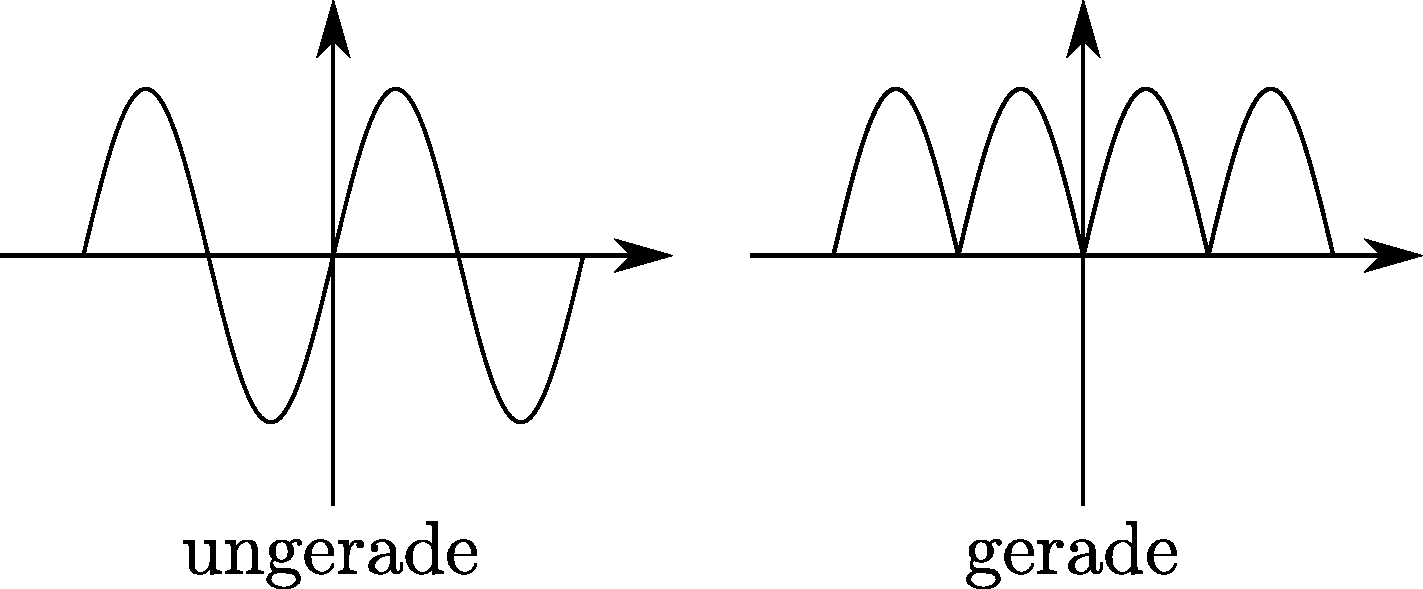
\includegraphics[width=0.7\textwidth]{geradeungerade.pdf}
\end{figure}

\subsection{n-te Partialsumme für die Periode T}\label{subsec:fouriert}
\[ \boxed{f_n(x) = \frac{a_0}{2} + \sum_{K=1}^n \left(a_k \cdot \cos \left(\frac{2 \pi}{T} K x\right) + b_k \cdot \sin\left(\frac{2 \pi}{T} K x\right)\right)} \]

\subsection{Koeffizienten für die Periode T}
\[ \boxed{a_k = \frac{2}{T} \int_T f(x) \cos(\frac{2 \pi}{T} K x) dx} \]
\[ \boxed{b_k = \frac{2}{T} \int_T f(x) \sin(\frac{2 \pi}{T} K x) dx} \]
\[ \boxed{a_0 = \frac{2}{T} \int_T f(x) dx
} \]
Ist $f$ eine ungerade Funktion d.h. $f(-x) = -f(x)$, so gilt, da der $\cos(x)$ eine gerade Funktion ist: 
\[ a_k \equiv 0 \quad \forall K\]
\[ a_0 \equiv 0 \]
Ist $f$ eine gerade Funktion: 
\[ b_k \equiv 0 \quad \forall K \]

\subsection{n-te Partialsumme einer Fourierreihe für die Periode 0 bis $2\pi$}\label{subsec:fourierpi}
Die folgende Fourierreihe besitzt eine Periode von 0 bis 2 $\pi$.
Sie ist ein Spezialfall der oben beschriebenen Variante.
\[ \boxed{f_n(x) = \frac{a_0}{2} + \sum_{K=1}^n \left(a_k \cdot \cos(kx) + b_k \cdot \sin(Kx)\right)} \]

\subsection{Koeffizienten für die Periode $2\pi$}
\[ \boxed{a_k = \frac{1}{\pi} \int_0^{2 \pi} f(x) \cos(nx) dx} \]
\[ \boxed{b_k = \frac{1}{\pi} \int_0^{2 \pi} f(x) \sin(nx) dx} \]
\[ \boxed{a_0 = \frac{1}{\pi} \int_0^{2 \pi} f(x) dx
} \]
Ist $f$ eine ungerade Funktion d.h. $f(-x) = -f(x)$, so gilt, da der $\cos(x)$ eine gerade Funktion ist: 
\[ a_k \equiv 0 \quad \forall K\]
\[ a_0 \equiv 0 \]
Ist $f$ eine gerade Funktion: 
\[ b_k \equiv 0 \quad \forall K \]

\subsection{Kochrezept zu Fourierreihen}
\begin{enumerate}
  \item Periode bestimmen\\
  Wenn die Periode $2\pi$ ist, kann die Formel für die Periode $2\pi$ (\ref{subsec:fourierpi} Seite \pageref{subsec:fourierpi}) verwendet werden. Ansonsten muss die Formel für die Periode T (\ref{subsec:fouriert} Seite \pageref{subsec:fouriert}) verwendet werden. 
  \item Funktion auf ganz $\mathbb{R}$ fortsetzen
  \item Bestimmung, ob gerade oder ungerade Funktion\\
  f ungerade: $a_0, a_k = 0$\\
  f gerade: $b_k = 0$
  \item $a_0, a_k$ und $b_k$ berechnen
  \item n-te trigonometrische Summe zu f hinschreiben
\end{enumerate}

\ifti
\subsection{Koeffizienzen der Fourierreihe mit dem TI-89 berechnen}
% \verb?integrate(?$\mathtt{\pi}$\verb?/2 * sin(@n1 * x),x,0,?$\mathtt{\pi}$\verb?)?\\
% $\mathtt{integrate\left(\frac{\pi}{2} \cdot sin(@n1 \cdot x), x, 0, \pi\right)}$\\
% $\text{integrate}\left(\frac{\pi}{2} \cdot \sin(@n1 \cdot x), x, 0, \pi\right)$
\verb?integrate(Ausdruck,Variable,untere Grenze, obere Grenze)? \\
\verb?integrate(EXPR,VAR[,LOW,UP])? \\\\
\begin{tabular}{@{}lll}
\verb?EXP?  & Ausdruck      & bezeichnet den Term der die Fourierreihe beschreibt \\
\verb?VAR?  & Variable      & bezeichnet die Variable, nach der integriert wird \\
\verb?LOW?  & untere Grenze & Anfangspunkt der Integration \\
\verb?HIGH? & obere Grenze  & Endpunkt der Integration \\
\end{tabular}\\
Für K wird \verb?@n1? eingegeben. 
\fi
\ifnspire
\subsection{Koeffizienten der Fourierreihe mit dem TI-Nspire berechnen}
\[ \int_{\boxed{a}}^{\boxed{b}}\boxed{\frac{\pi}{2}\sin(\mathtt{@n1} \cdot x)}~d\boxed{x} \]
a stellt hier die untere Grenze dar, b die obere Grenze.


Damit der Taschenrechner weiss, dass K eine natürliche Zahl zu sein hat (da es ja der Summenzähler ist), muss man K durch $\mathtt{@n1}$ ersetzen.


Das $\mathtt{@}$ findet man dabei bei den Symbolen (Taste $\boxed{\boxed{^{\infty \beta ^\circ}}}$)
\fi
